\documentclass[a4paper, 10pt]{article}

%% Language and font encodings
\usepackage[english]{babel}
\usepackage[utf8]{inputenc}
\usepackage[T1]{fontenc}

%% Sets page size and margins
\usepackage[a4paper,top=2.5cm,bottom=2.3cm,left=2.5cm,right=1.9cm]{geometry}


%% Useful packages
\usepackage{amsmath}
\usepackage{siunitx}
\usepackage{booktabs}
\usepackage{graphicx}
\usepackage[colorinlistoftodos]{todonotes}
\usepackage[colorlinks=true, allcolors=blue]{hyperref}
\usepackage{hyperref}
\usepackage{subcaption}
\usepackage{multirow}
\usepackage{arydshln}  % dashed lines
\usepackage{changepage}
\usepackage{blindtext} % lorem ipsum

\renewcommand{\arraystretch}{1.25} % for tables

\title{Your Paper}
\author{You}

\begin{document}
\maketitle
\newpage
\section{Lab 1}
  \subsection{Algorithm comparison}
  \begin{table}[h!]
    \begin{tabular}{@{}lrrrr@{}}
      \toprule
      \multicolumn{5}{c}{\textbf{gd}} \\
      N  &   $R_t$  &  $MSE_t$ &  Epch  & T(s)\\
      \midrule
      10       &   0.06     &  0.49       &  771     & 2.64   \\
      20       &   0.31     &  0.37       &  849     & 2.82   \\
      40       &   0.32     &  0.35       &  915     & 3.58   \\
      80       &   0.49     &  0.27       &  958     & 4.12   \\
      \hdashline
      100      &   0.48     &  0.53       &  976     & 4.90   \\
      120      &   0.47     &  0.62       &  957     & 7.15   \\
      \bottomrule
    \end{tabular} 
    \hfill
    \begin{tabular}{@{}lrrrr@{}}
      \toprule
      \multicolumn{5}{c}{\textbf{gda}} \\
      N  &   $R_t$  &  $MSE_t$ &  Epch  & T(s)\\
      \midrule
      10  & 0.17    & 0.51    & 79      &  0.28   \\
      20  & 0.25    & 0.48    & 79      &  0.53   \\
      40  & 0.29    & 0.54    & 67      &  0.58   \\
      80  & 0.22    & 0.88    & 68      &  0.59   \\                 
      \hdashline
      100 & 0.20    & 0.90    & 112     &  0.51   \\
      120 & 0.21    & 1.15    & 97      &  0.47   \\
      \bottomrule
    \end{tabular} 
    \hfill
    \begin{tabular}{@{}lrrrr@{}}
      \toprule
      \multicolumn{5}{c}{\textbf{cgf}} \\
      N  &   $R_t$  &  $MSE_t$ &  Epch  & T(s)\\
      \midrule
      10  & 0.15    & 0.50    & 11      &  0.10  \\
      20  & 0.42    & 0.38    & 17      &  0.31  \\
      40  & 0.65    & 0.28    & 30      &  0.54  \\
      80  & 0.69    & 0.29    & 44      &  0.53  \\
      \hdashline
     100  & 0.68    & 0.35    & 37      &  0.59  \\
     120  & 0.60    & 0.45    & 38      &  0.76  \\
      \bottomrule
    \end{tabular} 
    \mbox{}
    \begin{tabular}{@{}lrrrr@{}}
      \toprule
      \multicolumn{5}{c}{\textbf{cgp}} \\
      N  &   $R_t$  &  $MSE_t$ &  Epch  & T(s)\\
      \midrule
      10  & 0.17    & 0.48    & 12      &  0.10  \\
      20  & 0.33    & 0.48    & 15      &  0.40  \\
      40  & 0.60    & 0.32    & 25      &  0.48  \\
      80  & 0.67    & 0.31    & 35      &  1.59  \\
      \hdashline
     100  & 0.62    & 0.38    & 40      &  0.66  \\
     120  & 0.62    & 0.44    & 32      &  0.63  \\
      \bottomrule
    \end{tabular} 
    \hfill
    \begin{tabular}{@{}lrrrr@{}}
      \toprule
      \multicolumn{5}{c}{\textbf{bfg}} \\
      N  &   $R_t$  &  $MSE_t$ &  Epch  & T(s)\\
      \midrule
      10  & 0.18    & 0.48   & 11       & 0.15  \\
      20  & 0.43    & 0.40   & 17       & 0.30  \\
      40  & 0.77    & 0.20   & 35       & 0.86  \\
      80  & 0.91    & 0.9    & 39       & 2.34  \\
      \hdashline
     100  & 0.88    & 0.12   & 47       & 2.55  \\   
     120  & 0.75    & 0.28   & 47       & 3.59  \\
      \bottomrule
    \end{tabular} 
    \hfill
    \begin{tabular}{@{}lrrrr@{}}
      \toprule
      \multicolumn{5}{c}{\textbf{lm}} \\
      N  &   $R_t$  &  $MSE_t$ &  Epch  & T(s)\\
      \midrule
      10  & 0.18    & 0.44   & 11       & 0.07  \\ 
      20  & 0.50    & 0.38   &  6       & 0.10  \\ 
      40  & 0.85    & 0.13   & 11       & 0.18  \\ 
      \textbf{80} & \textbf{.93} & \textbf{.07}  & \textbf{6} & \textbf{.31} \\
      \hdashline
     100  & 0.90    & 0.10   & 4        & 0.26  \\
     120  & 0.81    & 0.22   & 5        & 0.27  \\  
      \bottomrule
    \end{tabular} \mbox{}
    \caption{Performance of different training algorithms. Results are the
      average ones after twenty runs on the test set. \emph{N} is the
      neurons on the hidden layer. $R_t$ and $MSE_t$ 
    stand for regression R-value and for MSE on the test set, respectively. 
    Test size is 15\% of the total data. \emph{Epch} stands for epoch of 
    convergence. \emph{T(s)} is time (seconds). Best result is 
    highlighted in bold. The dotted line separates overfitted results}
    \label{tab:train_algs}
  \end{table}

  \begin{figure}[h]
    \begin{adjustwidth}{-1.1cm}{-1.1cm}
    \centering
    \begin{subfigure}[t]{0.3\linewidth}
      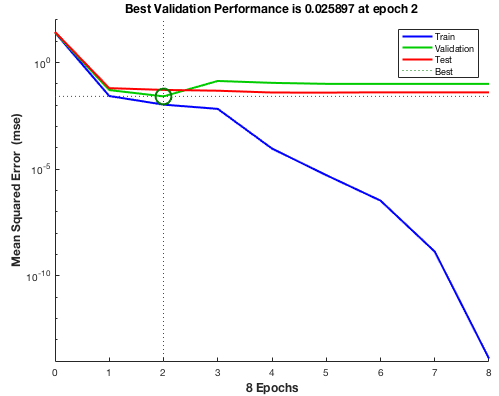
\includegraphics[width=1\linewidth]{./lab1/overfit_stop.png}
      \caption{Validation set avoids overfitting}
      \label{fig:perfect_fit}
    \end{subfigure}
    \begin{subfigure}[t]{0.3\linewidth}
      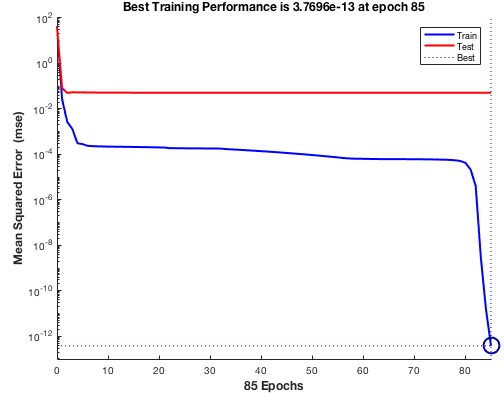
\includegraphics[width=1\linewidth]{./lab1/overfit.png}
      \caption{Overfit. 120 Neurons}
      \label{fig:overfit}
    \end{subfigure}
    \begin{subfigure}[t]{0.3\linewidth}
      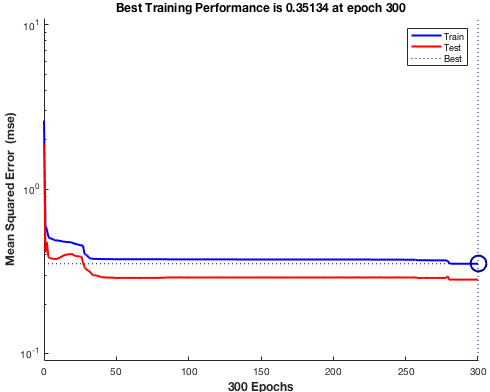
\includegraphics[width=1\linewidth]{./lab1/underfit.png}
      \caption{Underfit. 5 Neurons}
      \label{fig:underfit}
    \end{subfigure}
    \end{adjustwidth}
    \caption{Evolution of test (red), train (blue) and validation (green) set 
      MSE during training.  Left figure uses a validation set that stops befor
      e overfitting.  Otherwise, train error keeps sinking after the optima, a
      s \autoref{fig:overfit} also shows. On the right, with 5 neurons, the 
      training never converges: the net is too simple to learn the function, 
      error never decays. Test error (red) is lower than training error, it
      underfits.}
    \label{fig:validation}
  \end{figure}


  The goal here is comparing the six algorithms for training Neural Nets on
  the Matlab toolbox. For this purpose, I have trained a net using each 
  algorithm with different number of hidden units. Then, I have evaluated
  is performance on the test set, and repeated the process twenty times. 
  \autoref{tab:train_algs} shows the results of these experiments, averaged for
  each algorithm and neuron setting. Overall, all algorithms perform best
  with 80 hidden units: nets with neurons over that threshold 
  are overparametrized, since their MSE on the test set starts to decrease. 
  If there was no validation set, for 100 and 120 neurons the MSE on 
  train set would be way higher than that of test set, as
  \autoref{fig:validation} shows. On the other hand, nets with few hidden units
  do not even learn the model, and can have higher train error than test, as in
  \autoref{fig:underfit}.

  The best algorithm
  in terms of speed and performance is the \emph{Levenberg-Marquardt} (lm)
  algorithm: it trains the fastest and it reaches better performance
  than the other ones under the same configurations. \emph{Gradient descent}
  is by far the worst, both in speed and accuracy. The reason is that [maybe 
  that looks for the best option/not optimized -check]

  \subsubsection{Noisy data}
    \begin{figure}[h]
      \begin{adjustwidth}{-1.1cm}{-1.1cm}
      \centering
      \begin{subfigure}[t]{0.31\linewidth}
        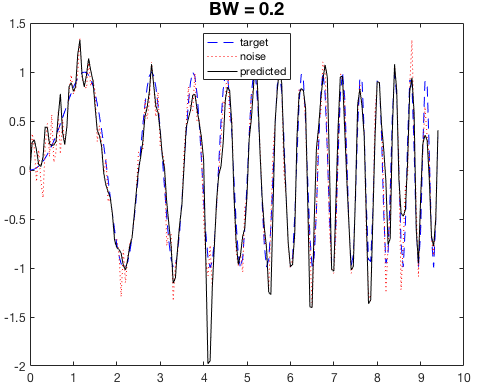
\includegraphics[width=1\linewidth]{./lab1/noise_2e-1.png}
        \caption{$R_t=0.54$, $MSE_t=0.53$}
        \label{fig:noise_small}
      \end{subfigure}
      \begin{subfigure}[t]{0.30\linewidth}
        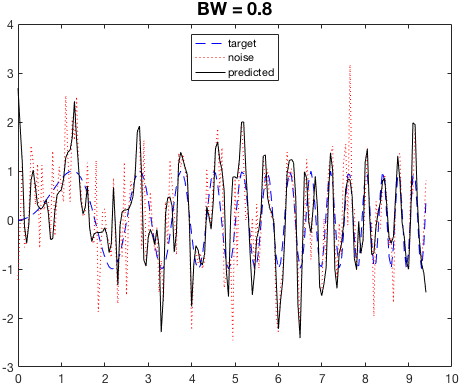
\includegraphics[width=1\linewidth]{./lab1/noise_8e-1.png}
        \caption{$R_t=0.38$, $MSE_t=2.25$}
        \label{fig:noise_big}
      \end{subfigure}
      \begin{subfigure}[t]{0.3\linewidth}
        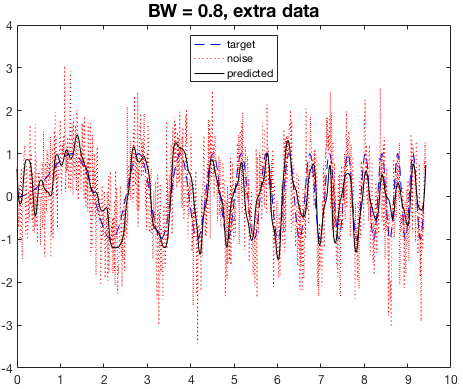
\includegraphics[width=1\linewidth]{./lab1/noise_8e-1_extra.png}
        \caption{$R_t=0.58$, $MSE_t=0.82$}
        \label{fig:noise_more_data}
      \end{subfigure}
      \end{adjustwidth}
      \caption{Estimation of a function with Gaussian noise, 0 mean, and different
        $\sigma$, or \emph{BW}. Figures (a) and (b) estimate on 190 data points, 
        figure (c) estimates on 950, 5 times more points. The network contains 80 
        hidden units, and it was trained using the \emph{lm} algorithm. MSE 
        with noisy data is worse, compared with the same setup on 
        \autoref{tab:train_algs}. Increasing the data points reduces again the 
        error, as (c) shows.}
      \label{fig:noise}
    \end{figure}

    \autoref{fig:noise} demonstrates that adding noise to the function affects
    the network estimation. It basically increases its error, no matter its
    setup. In this case, having more data points makes error go back to its
    original result: \autoref{fig:noise_more_data} shows it. This result 
    showcases another property of neural networks: they handle noisy data better
    than other estimators and even better when there is even more data, without
    increasing the demand for memory (opposed to SVM, where more data points mean
    bigger Kernel matrices).
      

  \subsection{Bayesian Inference}
  \begin{table}[h]
    \centering
    \hfill
    \begin{tabular}{@{}lrrrrr@{}}
      \toprule
      \multicolumn{6}{c}{\textbf{Levenberg-Marquardt}} \\
    N  &   $R_{t}$  &  $MSE_{t}$ &  $MSE_{tr}$ & Epch  & T(s)\\
      \midrule
      50   &   0.97    &   0.03    &  \num{0.81d-2}  &  8   &  0.15  \\
      100  &   0.90    &   0.10    &  \num{0.29d-2}  &  6   &  0.33  \\
      150  &   0.76    &   0.28    &  \num{0.01d-2}  &  5   &  0.31  \\
      300  &   0.41    &   1.00    &  \num{0.27d-2}  &  3   &  1.28  \\
      \bottomrule
    \end{tabular} 
    \hfill
    \begin{tabular}{@{}lrrrrr@{}}
      \toprule
      \multicolumn{6}{c}{\textbf{Bayesian Optimization}} \\
      N  &   $R_{t}$  &  $MSE_{t}$ & $MSE_{tr}$  & Epch  & T(s)\\
      \midrule
      50   &   1.00    &   \num{d-4}  &  \num{0.94d-7}   & 150   &    2.11  \\
      100  &   0.98    &   0.02       &  \num{0.50d-2}   & 106   &    6.52  \\
      150  &   0.89    &   0.11       &  \num{0.22d-4}   &  33   &   13.69  \\
      300  &   0.61    &   0.62       &  \num{0.19d-7}   &  27   &   92.65  \\
      \bottomrule
    \end{tabular}  \hfill\mbox{}
    \caption{Comparison between the Levenberg-Marquardt algorithm and Bayesian
    optimization, using overparametrized networks. $t$ stands for test set, $tr$
    stands for training set. As the hidden units increase, the \texttt{trainlm} 
    algorithm starts to overparametrize: validation set makes training finish 
    earlier and error on the test set increases too, whereas \emph{MSE} on the 
    training set remains constant. On the other hand, Bayes prior tries to keep
    the weights small, so test error increase is not as steep. In exchange, training
    takes more time, because finding the probabilities of each model takes
    much time.}
    \label{tab:bayes}
    \end{table}

    \autoref{tab:bayes} compares the performance of Bayesian learning against the 
    best performing algorithm from the previous section. The table showcases the
    main advantage of Bayesian optimization: it minimizes the weights of the
    network thanks to its prior distribution. Therefore, performance is better
    when there are too many hidden units. It comes at a price: training is way slower
    because there is no validation set; it calculates the probability distribution
    of the prior and the posterior at each level, which takes more time than regular
    backpropagation. The table also shows a common problem when searching the best
    parameter configuration: the \texttt{trainlm} algorithm reached its peak 
    performance with 50 neurons, but I skipped this setup on \autoref{tab:train_algs}




  





\newpage
\section{Lab 2}
  \subsection{Hopfield Network}
  Hopfield networks are recurrent NN with binary valued units that can store
  pattern according to the principles of associative memory, regarding storage
  capacity and retrieval. In this section I will illustrate their behaviour using
  them to retrieve original digits from noisy samples.

  \begin{figure}[h]
    \centering
    \includegraphics{lab2/digits/n1i10.png}
    \caption{}
    \label{fig:l2_no_noise}
  \end{figure}


  \newpage
\section{Unsupervised Learning}
  \subsection{Principal Component Analysis}
  \begin{figure}[h]
    \begin{adjustwidth}{-1cm}{-1cm}
    \centering
    \begin{subfigure}[t]{0.3\linewidth}
      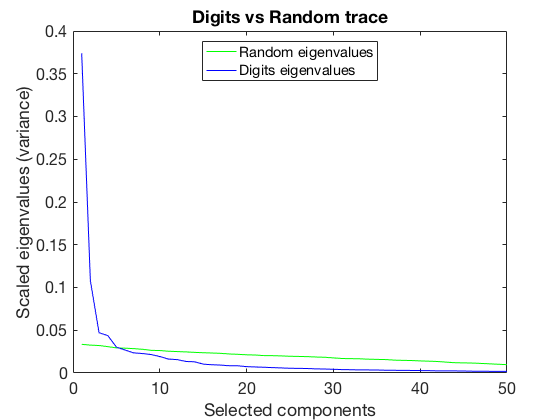
\includegraphics[width=1\linewidth, height=4.4cm]{./lab3/PCA/digits_vs_random_trace.png}
      \caption{Eigenvalues by PC}
      \label{fig:l3_traces}
    \end{subfigure}
    \begin{subfigure}[t]{0.29\linewidth}
      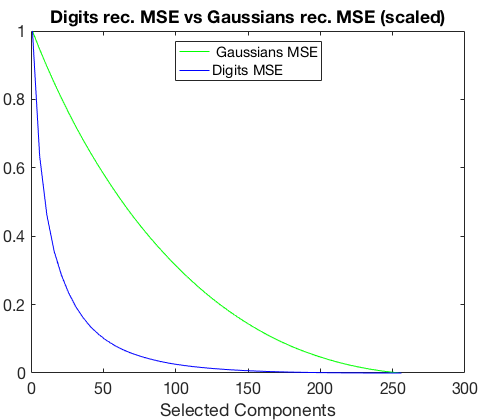
\includegraphics[width=1\linewidth, height=4.4cm]{./lab3/PCA/digits_vs_random_recMSE.png}
      \caption{Rec. \emph{MSE} by PC (scaled)}
      \label{fig:l3_rec_MSE}
    \end{subfigure}
    \begin{subfigure}[t]{0.3\linewidth}
      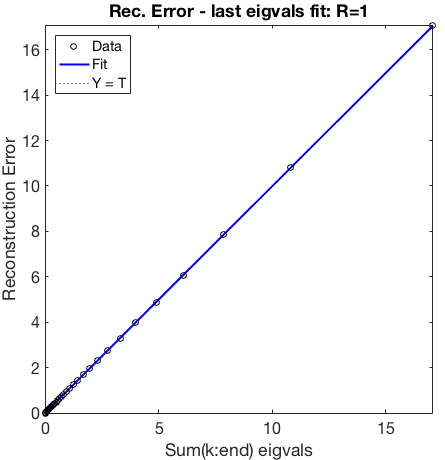
\includegraphics[width=1\linewidth, height=4.3cm]{./lab3/PCA/regression.png}
      \caption{Lin. fit: MSE and left-out variance}
      \label{fig:l3_regression}
    \end{subfigure}
    \end{adjustwidth}
    \caption{Comparison between a synthetic dataset (green) and the 
      \emph{threes} dataset, using their eigenvalues by PC (left) and their
      reconstruction error (centre, scaled by their max. value).
      Right image shows a perfect linear relation between recovery error and
      the summed variance of all the components but the first $k$ ones.}
    \label{fig:l3_first_task}
  \end{figure}

  The goal of this section is to understand the meaning and consequences of using
  PCA. \autoref{fig:l3_first_task} compares its behaviour on the \emph{threes} 
  dataset and on a random dataset of 256 I.d. Gaussian features. For the 
  \emph{threes} most information lies on the first PC: according to
  \autoref{fig:l3_traces}, 50 components explain already 90\% of the variance. On
  the Gaussians, that makes less than 40\%. Therefore, 50 components 
  should already deliver a good reconstruction of the digits, as 
  \autoref{fig:l3_rec_MSE} shows: MSE decreases steeply until then, and slowly 
  afterwards. On the other hand, on the Gaussian dataset information is 
  distributed evenly among the components. Both eigenvalues and MSE do not 
  decrease so sharply, there is no optimal transformation of the data such 
  that more information lies on a specific direction. 

  \begin{figure}[h]
    \centering
    \hfill
    \begin{subfigure}[t]{0.4\linewidth}
      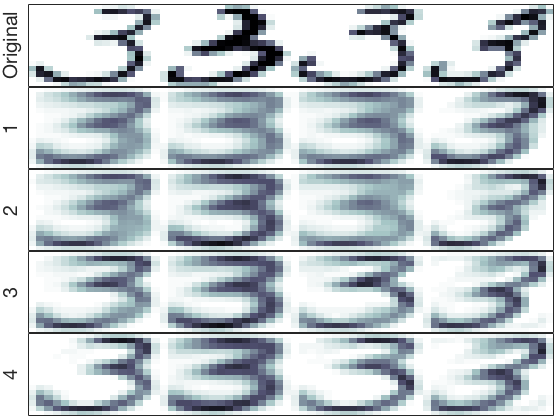
\includegraphics[width=\linewidth, height=4.3cm]{./lab3/PCA/mosaics/PC_1_4_small.png}
      %\caption{Few PC. $MSE(rec) > 0.9; variance < 12\%$}
      \label{fig:few_pc}
    \end{subfigure}
    \hfill
    \begin{subfigure}[t]{0.4\linewidth}
      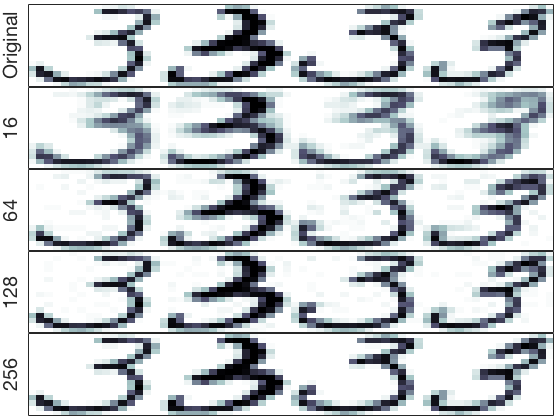
\includegraphics[width=\linewidth,height=4.3cm]{./lab3/PCA/mosaics/PC_16_256_small.png}
      %\caption{Many PC. $MSE(rec) < 0.75; variance > 45\%$}
      \label{fig:many_pc}
    \end{subfigure}
    \hfill \mbox{}
    \caption{Reconstruction of four different samples (columns) with increasing
      number of components (rows). Top row of each table contains the 
    original samples. Vertical labels indicate the number of components}
    \label{fig:l3_threes_pc}
  \end{figure}

  \paragraph{Visual reconstruction} a sample with few components 
  if much different from the original image, as the images on 
  \autoref{fig:l3_threes_pc} show. These recovered images seem more similar 
  to the average three. %TODO: put average three somewhere
  The reason is that the first components model the main structure underlying 
  all the data, the \emph{essence} of the \emph{threes}.
  As more components are added, reconstruction becomes more accurate.  The last 
  components model the noise, the particularities of each data point. Since
  most variance lies below 50 PC, any reconstruction with more PC delivers
  almost the same result, there is little margin of improvement. With
  With 256 PC the recovered image is exactly the same, and the \emph{MSE} is 0.
  %% maybe remove this
  There is a mathematical proof: being data $X \in {\rm I\!R}^{d \times N}$,
  with $d$ the input feature space; $V \in {\rm I\!R}^{d \times s}$ the
  eigenvector matrix, $s$ selected components; and $X_s=V^{t}X$ the data
  projected on those components. If $s=d$, then $VV^{t}=I$ (full rank orthogonal matrix).
  Then, $\hat{X} = VX_s = VV^{t}X = X$. 
  
  \begin{figure}[h]
    \centering
    \hfill
    \begin{subfigure}[t]{0.15\linewidth}
      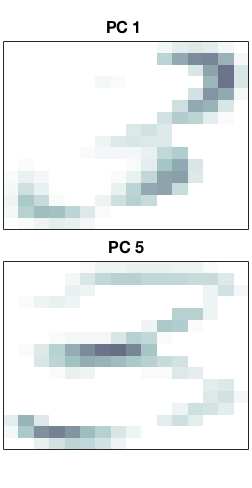
\includegraphics[width=\linewidth, height=5.5cm]{./lab3/PCA/PC_interpret/PC1+PC5.png}
    \end{subfigure}
    \hfill
    \begin{subfigure}[t]{5.4cm}
      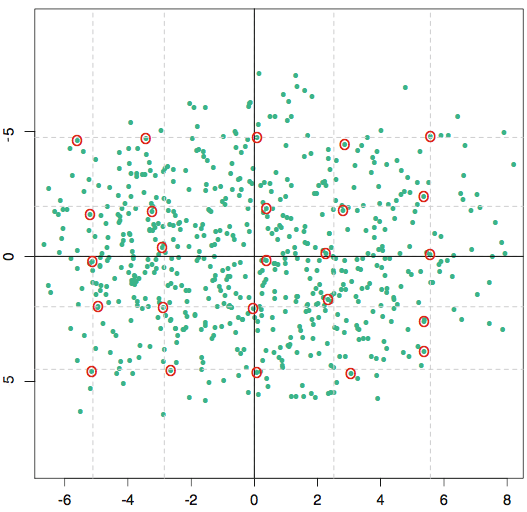
\includegraphics[width=\linewidth, height= 5.1cm]{./lab3/PCA/PC_interpret/quantiles.png}
    \end{subfigure}
    \hfill
    \begin{subfigure}[t]{5.4cm}
      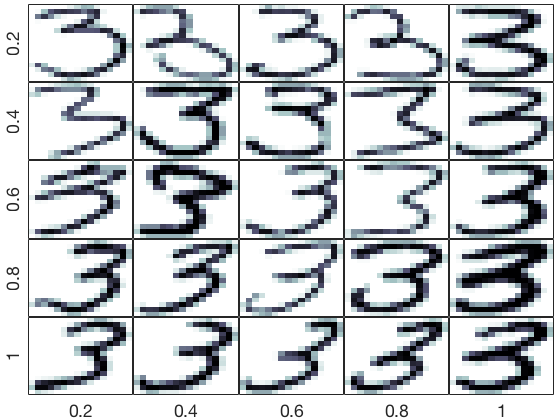
\includegraphics[width=\linewidth, height = 5.0cm]{./lab3/PCA/PC_interpret/Y1_X5.png}
    \end{subfigure}
    \hfill \mbox{}
    \caption{1st and 5th PC (left), and data points when projected on them 
    (centre). X axis correspond to the fifth, Y to the first. Red dots 
    show the closest data point to a quantile on the projections distribution.
    These samples are shown on the right image, with their corresponding quantile.}
    \label{fig:l3_pc_interpret}
  \end{figure}
  
  \paragraph{Component interpretation} each PC models data particularities, that
  can be used to find patterns on it, and even for clustering. 
  \autoref{fig:l3_pc_interpret} shows a representation of the first and fifth 
  component. Then, I have taken the points corresponding to different quantiles
  of the data, when projected on those components. The results are shown on the
  right image. PC 1 models cursiveness: threes on the Y axis lean to the left
  side on the low quantiles (top), and become totally cursive on the bottom rows.
  The fifth (X axis) models thickness on the horizontal strokes: digits at the 
  highest quantile (quantile) are the thickest.

  
  \subsection{Self Organizing Maps}
  %https://nl.mathworks.com/help/nnet/ug/cluster-with-self-organizing-map-neural-network.html
  \begin{figure}[h]
    \begin{adjustwidth}{-1cm}{-1cm}
    \centering
    \begin{subfigure}[t]{0.32\linewidth}
      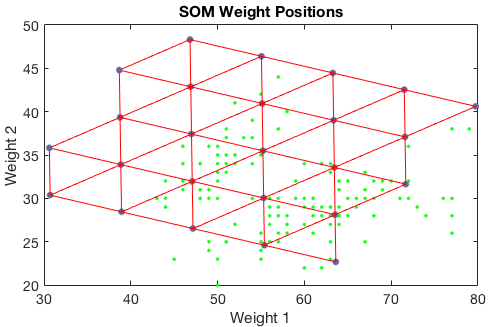
\includegraphics[width=1\linewidth]{./lab3/SOM/init_hex.png}
      \caption{Network initialization.}
      \label{fig:l3_init}
    \end{subfigure}
    \begin{subfigure}[t]{0.31\linewidth}
      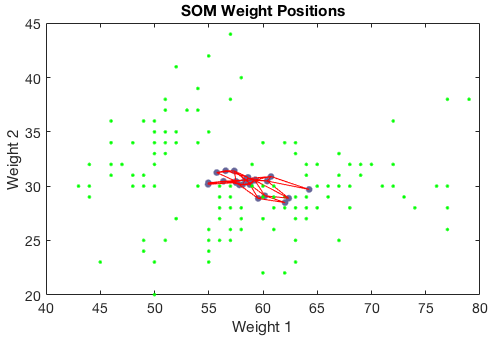
\includegraphics[width=1\linewidth]{./lab3/SOM/epoch1_hex.png}
      \caption{Training after one epoch}
      \label{fig:l3_epoch1}
    \end{subfigure}
    \begin{subfigure}[t]{0.31\linewidth}
      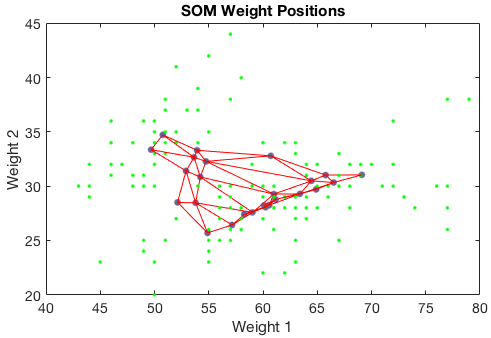
\includegraphics[width=1\linewidth]{./lab3/SOM/epoch5_hex.png}
      \caption{Final result}
      \label{fig:l3_epoch5}
    \end{subfigure}
    \end{adjustwidth}
    \caption{Training state evolution of a SOM with 25 neurons, set in a 
    hexagonal grid of $5\times5$. On the first epoch, many neurons
    are pulled together into the regions of high variance, since their 
    neighbourhood radius is very large. At later stages, neighbourhood size 
    shrinks and less neurons are pulled from their position.}
    \label{fig:l3_hex_grid}
  \end{figure}

  SOM deliver meaningful representations of the data (vector quantization) using
  competitive learning to make their neurons learn the data distribution. 
  Basically, as a neuron “wins” over the others for a data point, its weight is
  updated so it is closer to the input, according to the Konohen rule. In this 
  rule The new state depends on both the previous state and the input, and each
  has a different weight (parameter $\alpha$). Besides, neurons also pull their
  neighbours, defined by a radius on some distance metric and grid disposition. 
  \autoref{fig:l3_hex_grid} showcases the learning process of the SOM. Furthermore,
  they can also be used for clustering, with as many clusters as neurons. 
  \autoref{tab:l3_som_grid} compares clustering performance with different 
  configurations.

  \begin{table}[h]
    \centering
    \begin{tabular}{@{}llrrrrrrr@{}}
      \toprule
      & \phantom{ab}  & \texttt{linkdist} & \phantom{ab} & \texttt{dist} & 
      \phantom{ab} & \texttt{boxdist} & \phantom{ab} & \texttt{mandist} \\
      \midrule
      \textbf{Hexagonal} &&  $0.7240$  &&   $0.7240$  &&   $0.7254$  &&  $0.7239$\\
      \textbf{Grid}      &&  $0.7254$  &&   $0.7233$  &&   $0.7247$  &&  $0.7226$\\
      \textbf{Random}    &&  $0.6817$  &&   $0.7240$  &&   $0.7246$  &&  $0.7240$\\
      \bottomrule
    \end{tabular} 
    \caption{Comparison of different topologies and distances for the iris datset,
    using a $3 \times 1$ network for clustering. The displayed numbers correspond 
  to the ARI index.}
    \label{fig:l3_som_grid}
  \end{table}




    
    
    
    
    
    
    
    
    
\end{document}

